\section{Design}\label{Design}

\subsection{TAS Design}

TAS seeks to address a number of problems in the realm of datacenter packet
processing such as efficiency, predictability, and workload proportionality. 
Several important design decisions were made to accomplish these, but we will 
focus on just two of those: the split into a fast path and a slow path, and the
implementation of a userspace TCP stack.

One key way that TAS achieves high connection scalability and 
predictability is by dividing TCP functionality into two components: a fast 
path and a slow path. The fast path handles common-case packets and detects 
exceptions that need to be handled in the slow path. The main functions that
the fast path handles are common case send/receive, where the fast path directly
reads or writes packet payloads from application buffers and interacts directly
with the network; fast ACK handling, where the fast path will either generate or
consume ACK packets quickly without having to invoke the slow path; and 
efficient exception recognition and forwarding. 

In doing this, heavyweight TCP operations are taken out of the data path and 
relegated to the slow path, where they can be handled without affecting the 
performance of other flows in the fast path. The slow path does costly, 
infrequent operations like connection setup and teardown, timeouts, and 
enforcing congestion control. The slow path also handles out of order packets, 
but these are very infrequent in a datacenter environment.
   
In order for this separation and the individual components of the fast path 
and slow path to stay efficient, everything is implemented in a userspace TCP
stack. This provides all the normal functionality of TCP without having to 
switch back and forth between user and kernel space. This is good for 
performance and ease of programming, but isolates the TCP stack from Linux.
While we don't want to rely on Linux for performance-critical operations, it does contain
information about the network and a configurability that would be useful in a 
datacenter environment.

\subsection{Integration Goals}

To most effectively interface with Linux, we take advantage of the previously 
described TAS design choices in order to minimize our impact on common case
packet processing. 

First, we don't make any modifications to the fast path code or data structures.
We prioritize making changes around the fast path, but add no additional lines 
of code to common case packet processing, and no additions and minimal 
interaction with fast path data structures to avoid incurring contention, cache 
problems, or race conditions. By following this rule, we shouldn't incur any
direct overheads to the cases that we care most about.

Second, we don't worry about performance in the slow path as long as it
doesn't incur any scheduling or blocking problems with the fast path. We have 
very little control over how often Linux will deliver packets to the slow path, 
so we want to make sure this doesn't negatively affect the fast path threads 
when they might be co-scheduled with the slow path.

\subsection{Compromises Made}

In order to accomplish these goals, we made some compromises to certain problems
in our implementation. In these cases, we could have used fewer lines of code or 
perhaps gotten better performance for the slow path operation, but at the 
expense of potentially slowing down the fast path.

First, as previously discussed, the fast path naturally consumes all ACK packets,
including during connection setup. In order to most faithfully setup the 
connection, we would need to modify the fast path to either forward ACK packets 
to the slow path, or write packets directly to the tap device. Instead of 
absorbing these costs in the fast path, we instead manually create a new ACK
packet during connection setup in the slow path and write it to the tap device.

Second, we maintain separate sequence numbers between Linux and TAS and 
between TAS and remote hosts. TAS immediately initializes fast path 
state upon receiving a \textit{SYN} packet and doesn't update it after that unless 
there is some kind of exception. Although this takes place in the slow path,
this would require adding some kind of complexity, as we won't know the sequence
number Linux wants to use until it provides a \textit{SYN/ACK}. We can address this by 
doing one of the following: adding an artificial delay or some kind of signal 
from the thread interacting with Linux in the middle of \textit{SYN} processing to make 
sure the sequence number is available when fast path state is initialized, 
initializing fast path state at a later time, modifying the fast path to 
identify either outgoing \textit{SYN/ACK} packets or incorrect outgoing sequence numbers
and adapting, or keeping separate sequence numbers. The final solution ended up 
being the simplest; the first will slow down connection setup even more, the 
second may create additional race conditions or problems in connection setup, 
and the third will slow down the fast path in some way.

Third, similarly to the first compromise, we handle ARP packets manually in 
the slow path, as they are not always forwarded to the slow path. By default,
the fast path only forwards ARP packets to the slow path if it is an IP address
that it doesn't have state for. As connection state is initialized immediately 
upon a \textit{SYN} packet being received, if we try to forward any Linux ARPs to the 
network for that connection, the replies will be dropped by the fast path. In
this case, instead of forwarding all ARP packets to the slow path or delaying
initializing connection state again, we fake ARP responses to Linux requests 
in the slow path by searching TAS's ARP table and manually crafting 
packets. 

\begin{figure}
\centering
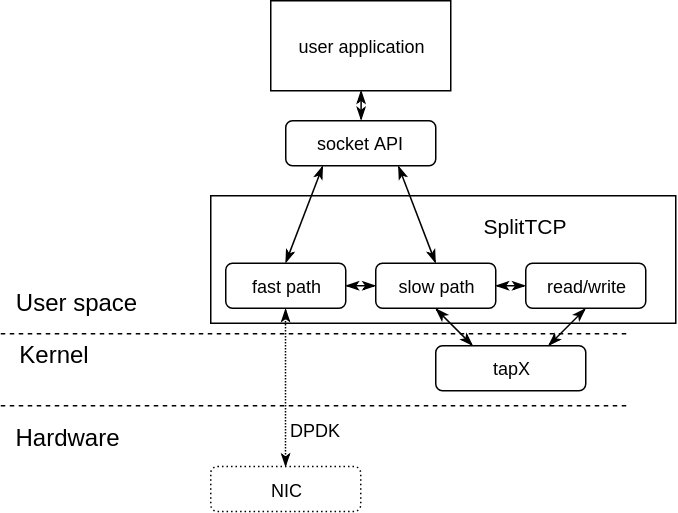
\includegraphics[width=0.7\columnwidth]{figures/splittcp.png}
\caption{Design of TAS with kernel integration. TAS now replicates all slow path operations to the kernel, checks what
it did by reading raw packets from the TAP device and mimics its decisions.}
\label{fig:splittcp_tap}
\end{figure}
